\section{Objectives and specification mapping}
Lab 13 (PDF pages 55--57) compares static CMOS and pseudo NMOS inverters. Step 1 retains a 500 MHz input and sweeps PMOS/NMOS width ratio. Step 2 changes size and output load, measuring a usable-frequency bracket and average power at the highest passing point. A separate DC sweep isolates low-level error and static loss. All four netlists and 116 cases solved and measured successfully.

\section{Circuit and acceptance criterion}
Both circuits use an NMOS pull-down. The CMOS PMOS gate follows the input; the pseudo NMOS PMOS gate is fixed at 0 V and therefore stays on. Baseline dimensions are $W_n=0.6\,\mu$m, $W_p=0.9\,\mu$m and $L=0.25\,\mu$m, with 7 fF load. Width ratios are 0.25/0.5/1/1.5/3/6. Size/load pairs are (1,7 fF), (2,7 fF), (1,14 fF) and (2,14 fF).

A fixed explicit criterion defines usable frequency: settled sampled low level at most 0.3 V and high level at least 0.7 V. The initial 0.1--10 GHz scan is refined to a 0.1 GHz passing/failing bracket. This is a bracket for this sampling convention and load, not a device rating valid for every receiver, nor an exact maximum on a continuous frequency axis.

\section{Simulation setup and measurement definitions}
The separately supplied MOS model is evaluated at 1.0 V and $27\,^{\circ}$C, retaining the handout topology and the comparison conditions below. One volt is a simulation setting, not a device rating established by available model documentation. Numerical results from the handout's older processes are not acceptance targets for this model.

HSPICE S-2021.09 runs with RUNLVL=6. Tables use actual native measurements and figures use actual printed numerical traces. Every variant resets all swept parameters and temperature, avoiding inherited settings from an earlier variant. Completed solutions and measurements do not establish process reliability. Internal warnings in encrypted model blocks remain incompletely visible.
Each input begins rising at $0.25T$, with rise/fall parameters $0.01T$ and a high pulse width $0.48T$. Twelve periods are simulated with 500 printed points per period. Low and high outputs are sampled at $10.7T$ and $11.2T$; supply power is averaged from period 4 to period 12. Separate ideal supplies isolate the two circuits, with positive supply power defined as $P=-\overline{V_{DD}I(V_{DD})}$.

\section{Width-ratio and static results}
The table uses 500 MHz, size 1 and 7 fF. Powers are in $\mu$W.

\begin{center}\small
\begin{tabular}{llllll}
\toprule
$W_p/W_n$ & CMOS $V_L$ & Pseudo $V_L$ & Pseudo $V_H$ & CMOS P & Pseudo P \\
\midrule
0.25 & 0.0000 & 0.0110 & 0.8140 & 3.700 & 7.823 \\
0.5 & 0.0000 & 0.0232 & 0.9910 & 4.441 & 12.783 \\
1 & 0.0000 & 0.0485 & 1.0000 & 4.810 & 21.706 \\
1.5 & 0.0000 & 0.0755 & 1.0000 & 5.156 & 30.540 \\
3 & 0.0000 & 0.1709 & 1.0000 & 6.138 & 56.405 \\
6 & 0.0000 & 0.5860 & 1.0000 & 7.918 & 92.040 \\
\bottomrule
\end{tabular}
\end{center}
\begin{figure}[htbp]
\centering
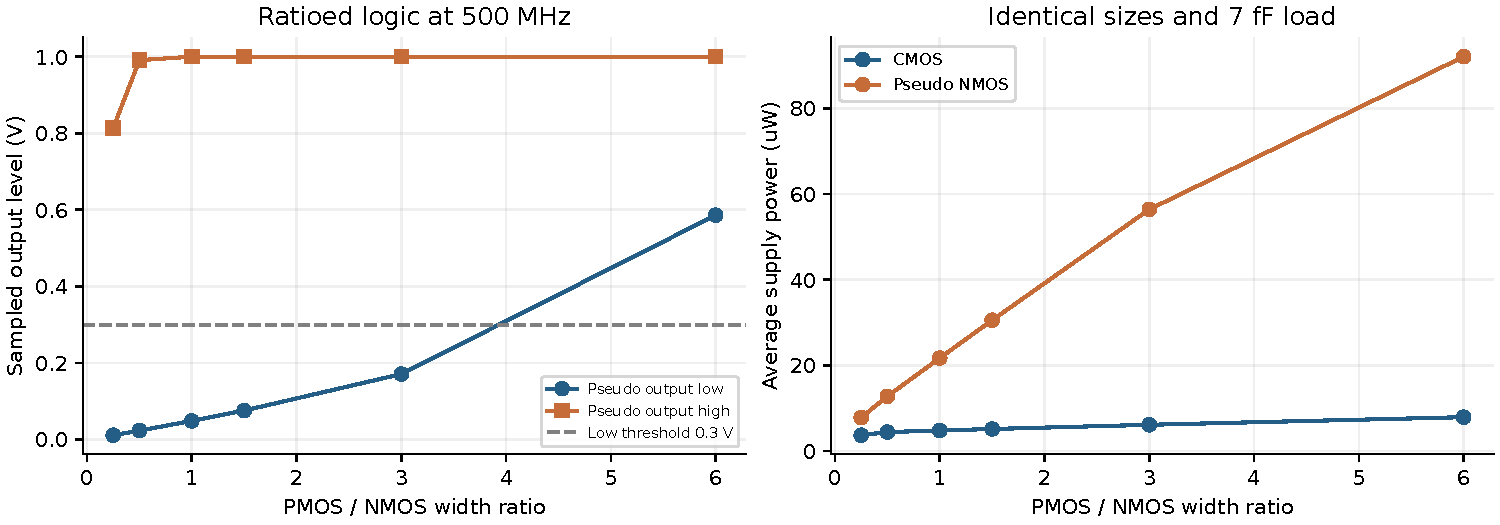
\includegraphics[width=\linewidth]{figures/pseudo_ratio.pdf}
\caption{The always-on pull-up makes level and power ratio-dependent; ratio 6 fails the low-level criterion.}
\end{figure}
At a DC 1 V input, the CMOS output is 3.88 $\mu$V, while pseudo NMOS produces 0.07550 V and draws 54.548 $\mu$A of static supply current. This is the sustained low-output current; average static power also depends on the time spent in that input state.
\section{Highest passing frequency and power}
The lower bound passes and the adjacent upper bound fails. Power is measured at the passing lower bound.

\begin{center}\small
\begin{tabular}{lllll}
\toprule
Size & Load (fF) & Logic & Pass / fail (GHz) & P ($\mu$W) \\
\midrule
1 & 7 & CMOS & 3.0 / 3.1 & 25.302 \\
1 & 7 & Pseudo NMOS & 3.8 / 3.9 & 50.583 \\
2 & 7 & CMOS & 4.5 / 4.6 & 50.934 \\
2 & 7 & Pseudo NMOS & 6.0 / 6.1 & 101.683 \\
1 & 14 & CMOS & 1.8 / 1.9 & 24.942 \\
1 & 14 & Pseudo NMOS & 2.2 / 2.3 & 50.658 \\
2 & 14 & CMOS & 3.0 / 3.1 & 50.741 \\
2 & 14 & Pseudo NMOS & 3.8 / 3.9 & 101.784 \\
\bottomrule
\end{tabular}
\end{center}
\begin{figure}[htbp]
\centering
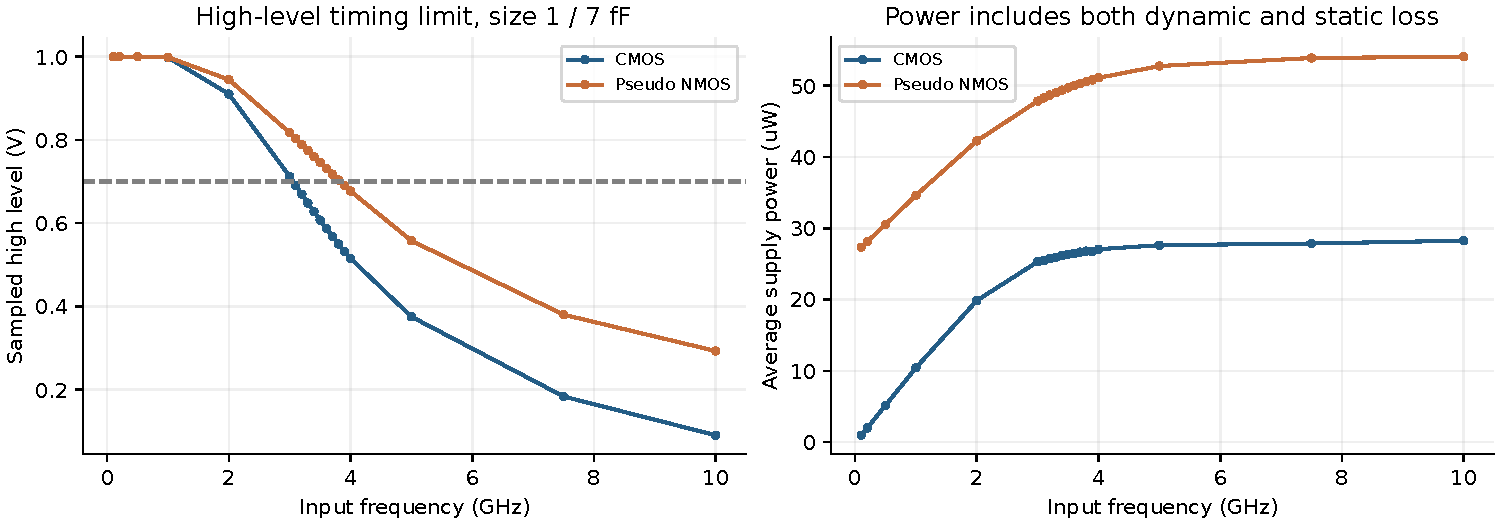
\includegraphics[width=\linewidth]{figures/pseudo_frequency.pdf}
\caption{High level and average power for size 1 / 7 fF. Failing points remain visible to show the timing limit.}
\end{figure}
\section{Discussion and questions}
At size 1 and 7 fF, CMOS passes through 3.0 GHz and fails at 3.1 GHz; pseudo NMOS passes through 3.8 GHz and fails at 3.9 GHz. Larger devices improve this range but increase always-on current, while doubling load reduces usable frequency. Both low- and high-level criteria remain enforced; a small pseudo NMOS oscillation is not automatically accepted as useful logic.

For one charge/discharge event per period, approximate CMOS dynamic power is $fCV_{DD}^{2}$, while pseudo NMOS power is $fCV_{DD}V_{swing}+\overline{I_{DC}}V_{DD}$. Ignoring other contributions, pseudo NMOS can consume less only if $\overline{I_{DC}}<fC(V_{DD}-V_{swing})$. This conditional comparison does not guarantee lower power at high frequency. Pseudo NMOS consumes more in the equal-size/equal-load tests here. Power flattening after logic-level failure is not an efficiency benefit under valid operation.

Two-input NAND/NOR cores use four devices in static CMOS and three in pseudo NMOS; general n-input forms use approximately $2n$ versus $n+1$. Actual area still depends on widths, contacts and routing, so no layout-area claim follows. Each pseudo NMOS input drives only the pull-down network, reducing input loading at the cost of a DC path, elevated low level and sizing-ratio dependence. A NAND's series NMOS path must still overcome the always-on PMOS. A pseudo NOR replaces the series PMOS pull-up with one PMOS, but recovery to high remains limited by that pull-up. These are structural arguments, not an additional measured NAND/NOR speed ranking.

\section{Reproducibility files}
Netlists: \texttt{01\_ratio.sp}, \texttt{02\_frequency.sp}, \texttt{03\_dc\_power.sp}, \texttt{04\_frequency\_refinement.sp}. Add the local model configuration at the marked comment before execution; model files and paths are omitted from the public files.

The results directory contains all case measurements, derived metrics, the specification manifest and representative waveform CSVs. Waveforms retain at most 2501 uniformly selected samples; measurements are not downsampled. Full listings remain local.
